%%% chapter1.tex ---Глава 1
\section{Актуальность проблемы стеганографической передачи данных в современной кибербезопасности}

\subsection{Анализ современного ландшафта киберугроз}

Современный ландшафт киберугроз характеризуется высокой динамикой и развитием сложных методов атак. Согласно отчётам компаний Positive Technologies, Kaspersky и Group-IB за период 2024–2026 годов, наблюдается рост числа инцидентов, связанных с утечками данных и проникновениями в корпоративные сети на 20–30\,\% ежегодно~[11, 12, 13]. Среди ключевых угроз выделяются следующие классы:

\begin{enumerate}[label=\arabic*)]
    \item участники продвинутых постоянных угроз (APT-группировки), использующие скрытные техники проникновения и длительного тайного присутствия в сети;
    \item вредоносное программное обеспечение-вымогатели (ransomware), наносящее существенный ущерб информационным системам;
    \item промышленный шпионаж, направленный на похищение интеллектуальной собственности и коммерческих тайн.
\end{enumerate}

Динамика роста числа значимых инцидентов информационной безопасности за период 2019--2024 годов наглядно демонстрирует масштаб проблемы. На рисунке~\ref{fig:incident_dynamics} представлена сравнительная статистика инцидентов в глобальном масштабе и в российском сегменте. Данные основаны на ежегодных отчётах Positive Technologies за указанный период~[11].

\begin{figure}[htbp]
    \centering
    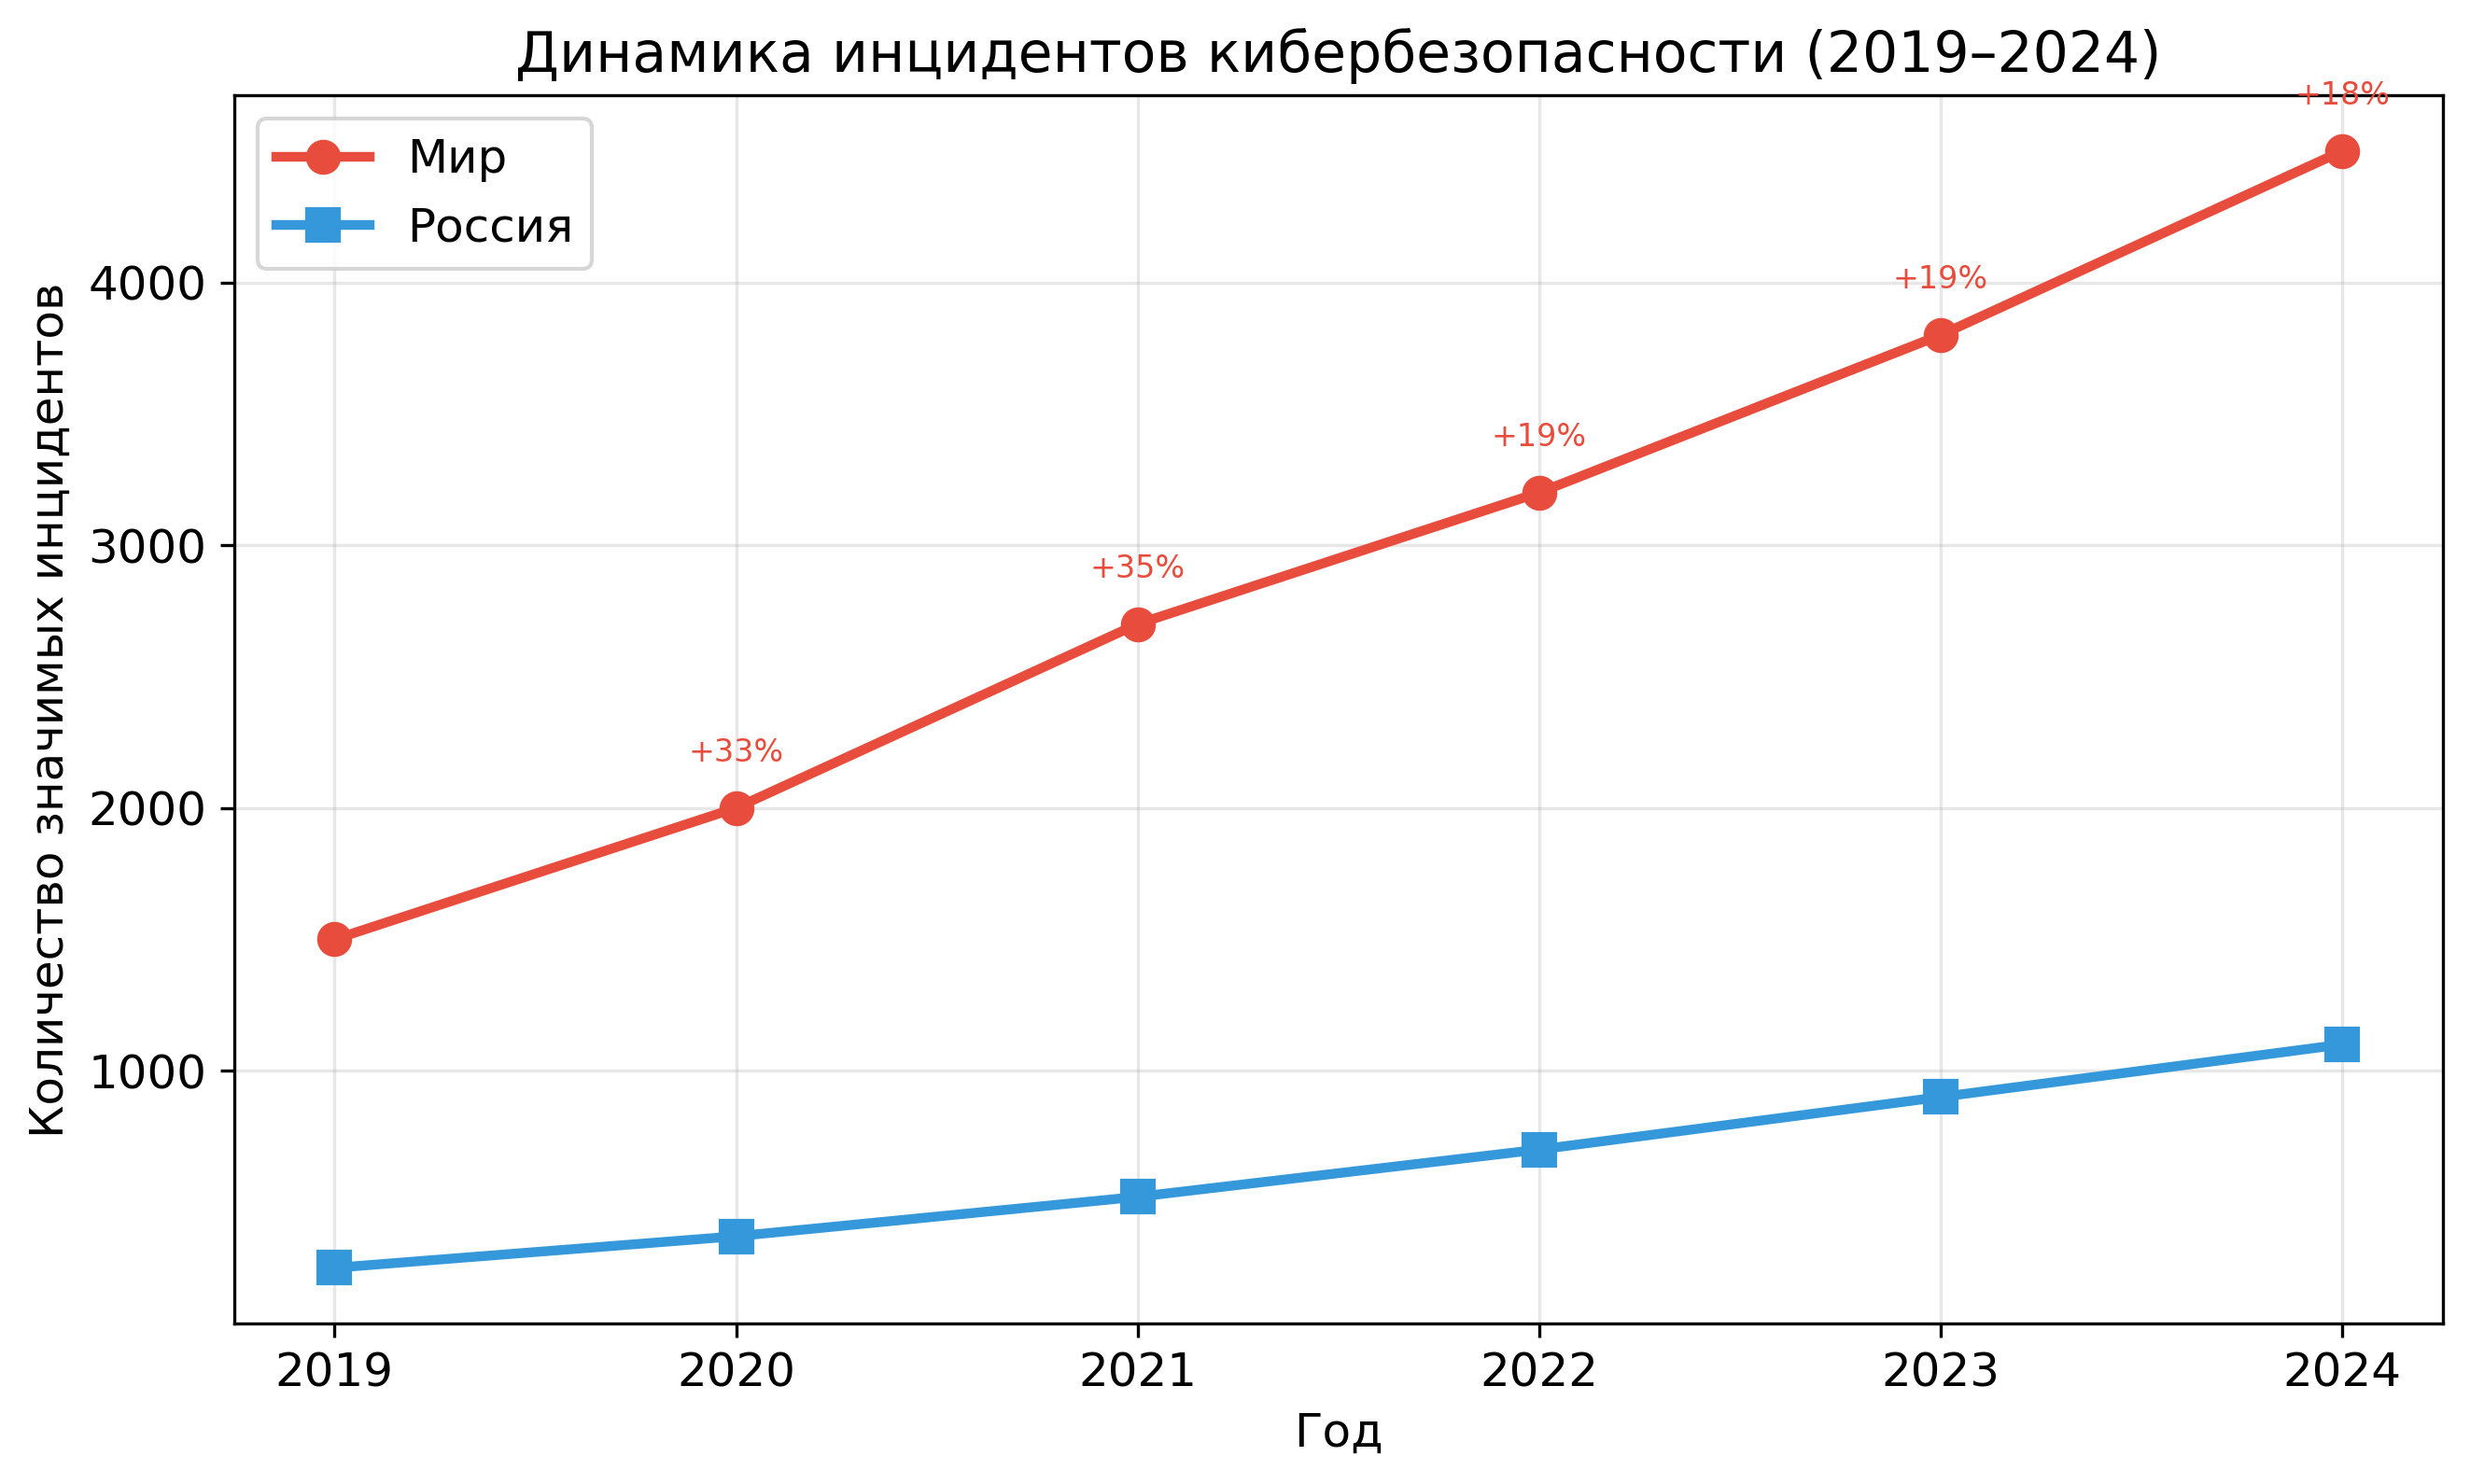
\includegraphics[width=0.85\textwidth]{images/incident_dynamics.png}
    \caption{Динамика инцидентов кибербезопасности (2019--2024)}
    \label{fig:incident_dynamics}
\end{figure}

Как видно из графика, количество значимых инцидентов в мире выросло с~1500 в 2019~году до~4500 в 2024~году, что составляет трёхкратное увеличение за пятилетний период. В российском сегменте наблюдается ещё более выраженная динамика~--- рост с~250 до~1100 инцидентов, то есть более чем в четыре раза. Данная тенденция обусловлена, в частности, геополитическими факторами, усилением активности хактивистских группировок и целенаправленными атаками на объекты критической информационной инфраструктуры Российской Федерации~[12, 13].

Анализ структуры кибератак по типам позволяет выделить наиболее распространённые векторы угроз. На рисунке~\ref{fig:attack_types} представлено распределение типов атак по данным аналитического отчёта Positive Technologies за 2024~год.

\begin{figure}[htbp]
    \centering
    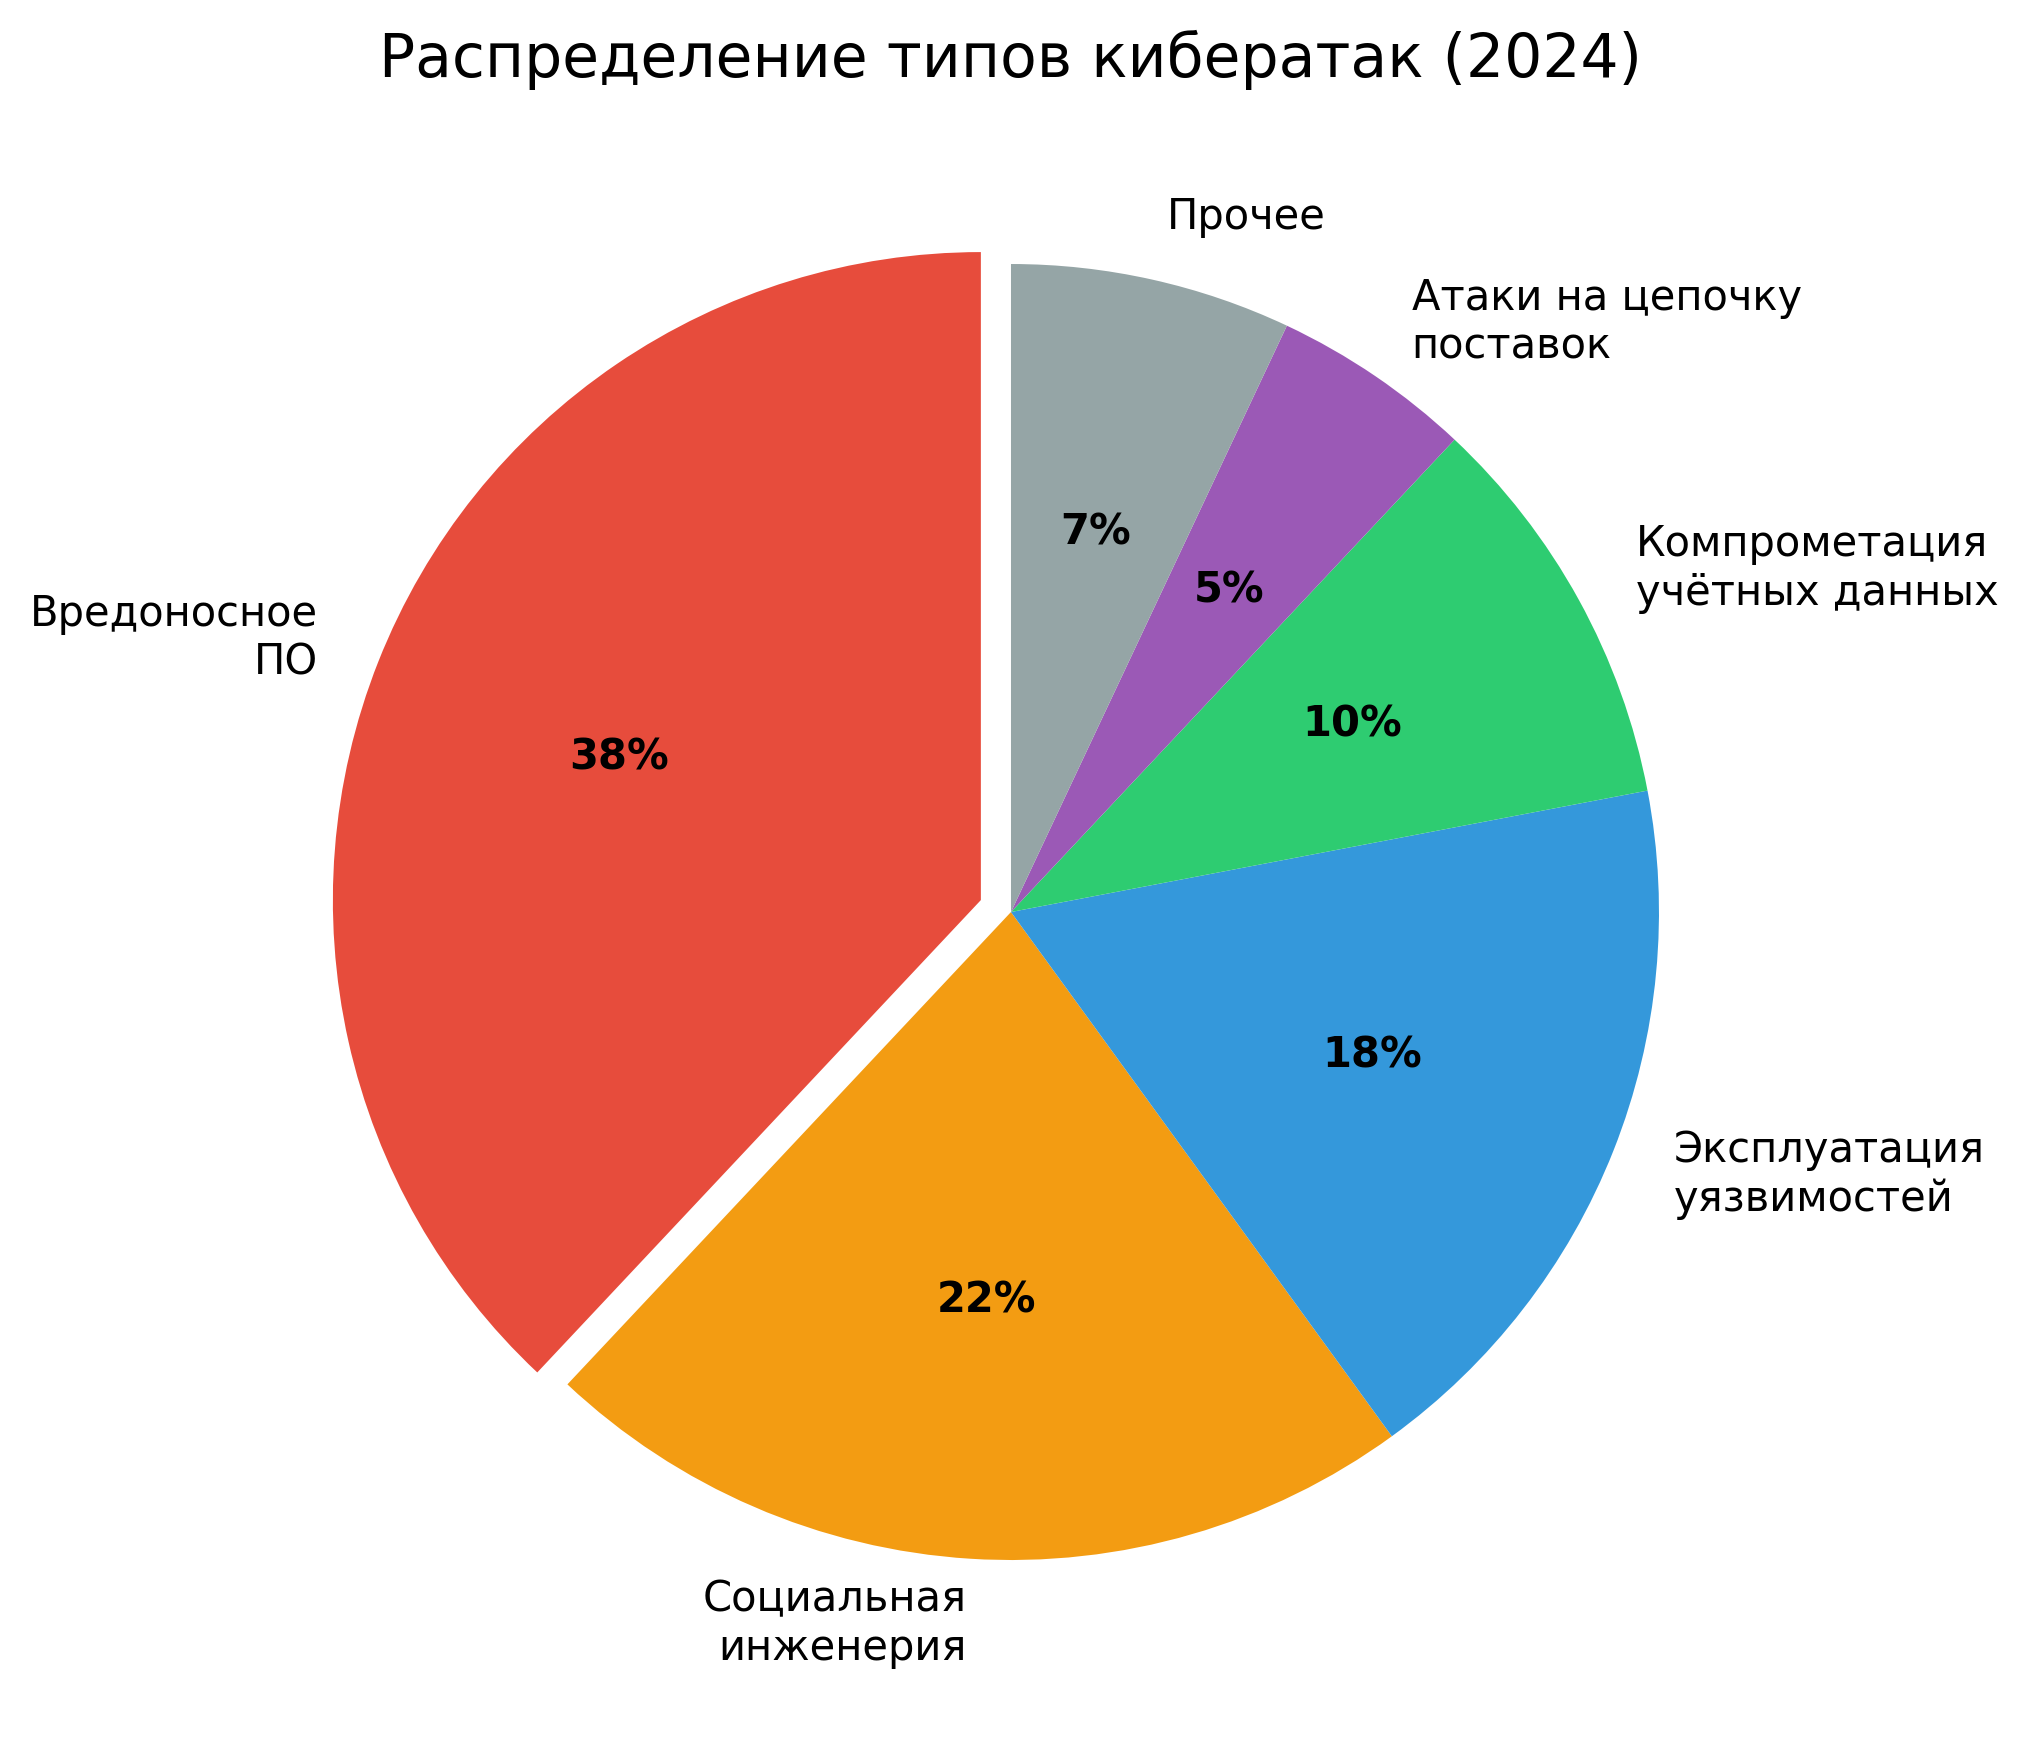
\includegraphics[width=0.75\textwidth]{images/attack_types.png}
    \caption{Распределение типов кибератак (2024)}
    \label{fig:attack_types}
\end{figure}

Доминирующим типом атак остаётся вредоносное программное обеспечение (38\,\%), включающее ransomware, трояны и бэкдоры. Социальная инженерия занимает второе место (22\,\%), что подчёркивает значимость человеческого фактора в обеспечении информационной безопасности. Эксплуатация уязвимостей программного обеспечения составляет 18\,\% инцидентов, что связано с ростом числа обнаруживаемых уязвимостей нулевого дня. Атаки на цепочку поставок (5\,\%), несмотря на относительно малую долю, характеризуются высоким потенциалом ущерба, поскольку позволяют компрометировать множество организаций через единую точку входа.

Важной тенденцией является переход от явных атак и массовых сканирований к методам low-and-slow, в рамках которых злоумышленники стремятся оставаться незаметными за счёт снижения интенсивности активности и использования стеганографических каналов передачи команд и контрольных сообщений~[11]. Это ставит новые задачи для систем киберзащиты, требующих развития механизмов выявления скрытых угроз.

\subsection{Тенденции применения стеганографии злоумышленниками}

Стеганография, как техника скрытия информации внутри иных носителей, издавна использовалась в военных и разведывательных целях, однако с развитием компьютерных технологий и сетей стала инструментом для киберпреступников. Исторические примеры применения сетевой стеганографии включают вредоносные программы Duqu и Flame~[14], а также проект ProjectSauron~[15], где была задокументирована реализация скрытых командных каналов. Современные кейсы, такие как деятельность группировки Turla, демонстрируют использование DNS-запросов в качестве стеганографического канала~[11], а также расследования Equation Group показывают сложные методы встраивания информации в TCP/IP стек~[16].

Более детальный анализ деятельности указанных группировок позволяет оценить масштаб и техническую сложность применяемых стеганографических методов. Группировка Turla (также известная как Snake, Venomous Bear, Uroburos), связываемая аналитиками с российскими спецслужбами, разработала один из наиболее изощрённых механизмов DNS-туннелирования. Вредоносное ПО данной группы формировало DNS-запросы к контролируемым злоумышленниками серверам имён, кодируя команды и эксфильтрируемые данные в полях QNAME с использованием кастомного алфавита Base64. Ключевой особенностью являлось использование легитимных DNS-резолверов организации-жертвы в качестве промежуточных узлов, что позволяло обходить ограничения межсетевого экрана на прямые DNS-запросы к внешним серверам~[11]. Для снижения вероятности обнаружения система ограничивала частоту запросов до 1--2 в минуту и варьировала длину QNAME, имитируя паттерны обращений к CDN-сервисам.

Группировка Equation Group, описанная в отчётах компании Kaspersky~[16], применяла модификацию полей TCP/IP стека для организации скрытых каналов управления имплантами. В частности, было задокументировано использование поля IP Identification для передачи однобайтовых команд, а также манипуляция порядковыми номерами TCP для кодирования четырёхбайтовых блоков данных. Особый интерес представляет применение данной группировкой техники <<двойного дна>>: первичный канал связи осуществлялся через HTTP, а стеганографический канал в TCP ISN активировался только при получении специальной команды-триггера, что существенно затрудняло его обнаружение при ретроспективном анализе трафика.

Вредоносное ПО StegoLoader, впервые обнаруженное исследователями Dell SecureWorks, представляет пример гибридного подхода: основной модуль загрузки использовал стеганографию в PNG-изображениях для доставки полезной нагрузки, однако командно-контрольный канал был реализован через манипуляцию полями ICMP Echo Request. Размер полезной нагрузки ICMP-пакетов варьировался в пределах 56--84~байт, что соответствовало типичным значениям для утилиты \texttt{ping} различных ОС, а данные размещались в последних 8--16~байтах payload.

Группировка APT29 (Cozy Bear) в рамках кампании Hammertoss использовала многоуровневую стеганографическую схему: управляющие команды кодировались в изображениях, публикуемых на платформе Twitter (ныне X), а адреса серверов для эксфильтрации извлекались из временных меток публикаций. Данный подход демонстрирует тенденцию к использованию легитимных социальных платформ в качестве промежуточного звена стеганографической коммуникации, что существенно усложняет блокировку C2-каналов на уровне сетевой инфраструктуры.

Обобщённая характеристика APT-группировок, применяющих стеганографические техники, представлена на рисунке~\ref{fig:apt_stego}. Диаграмма отражает продолжительность известной активности каждой группировки и используемые ею стеганографические методы.

\begin{figure}[htbp]
    \centering
    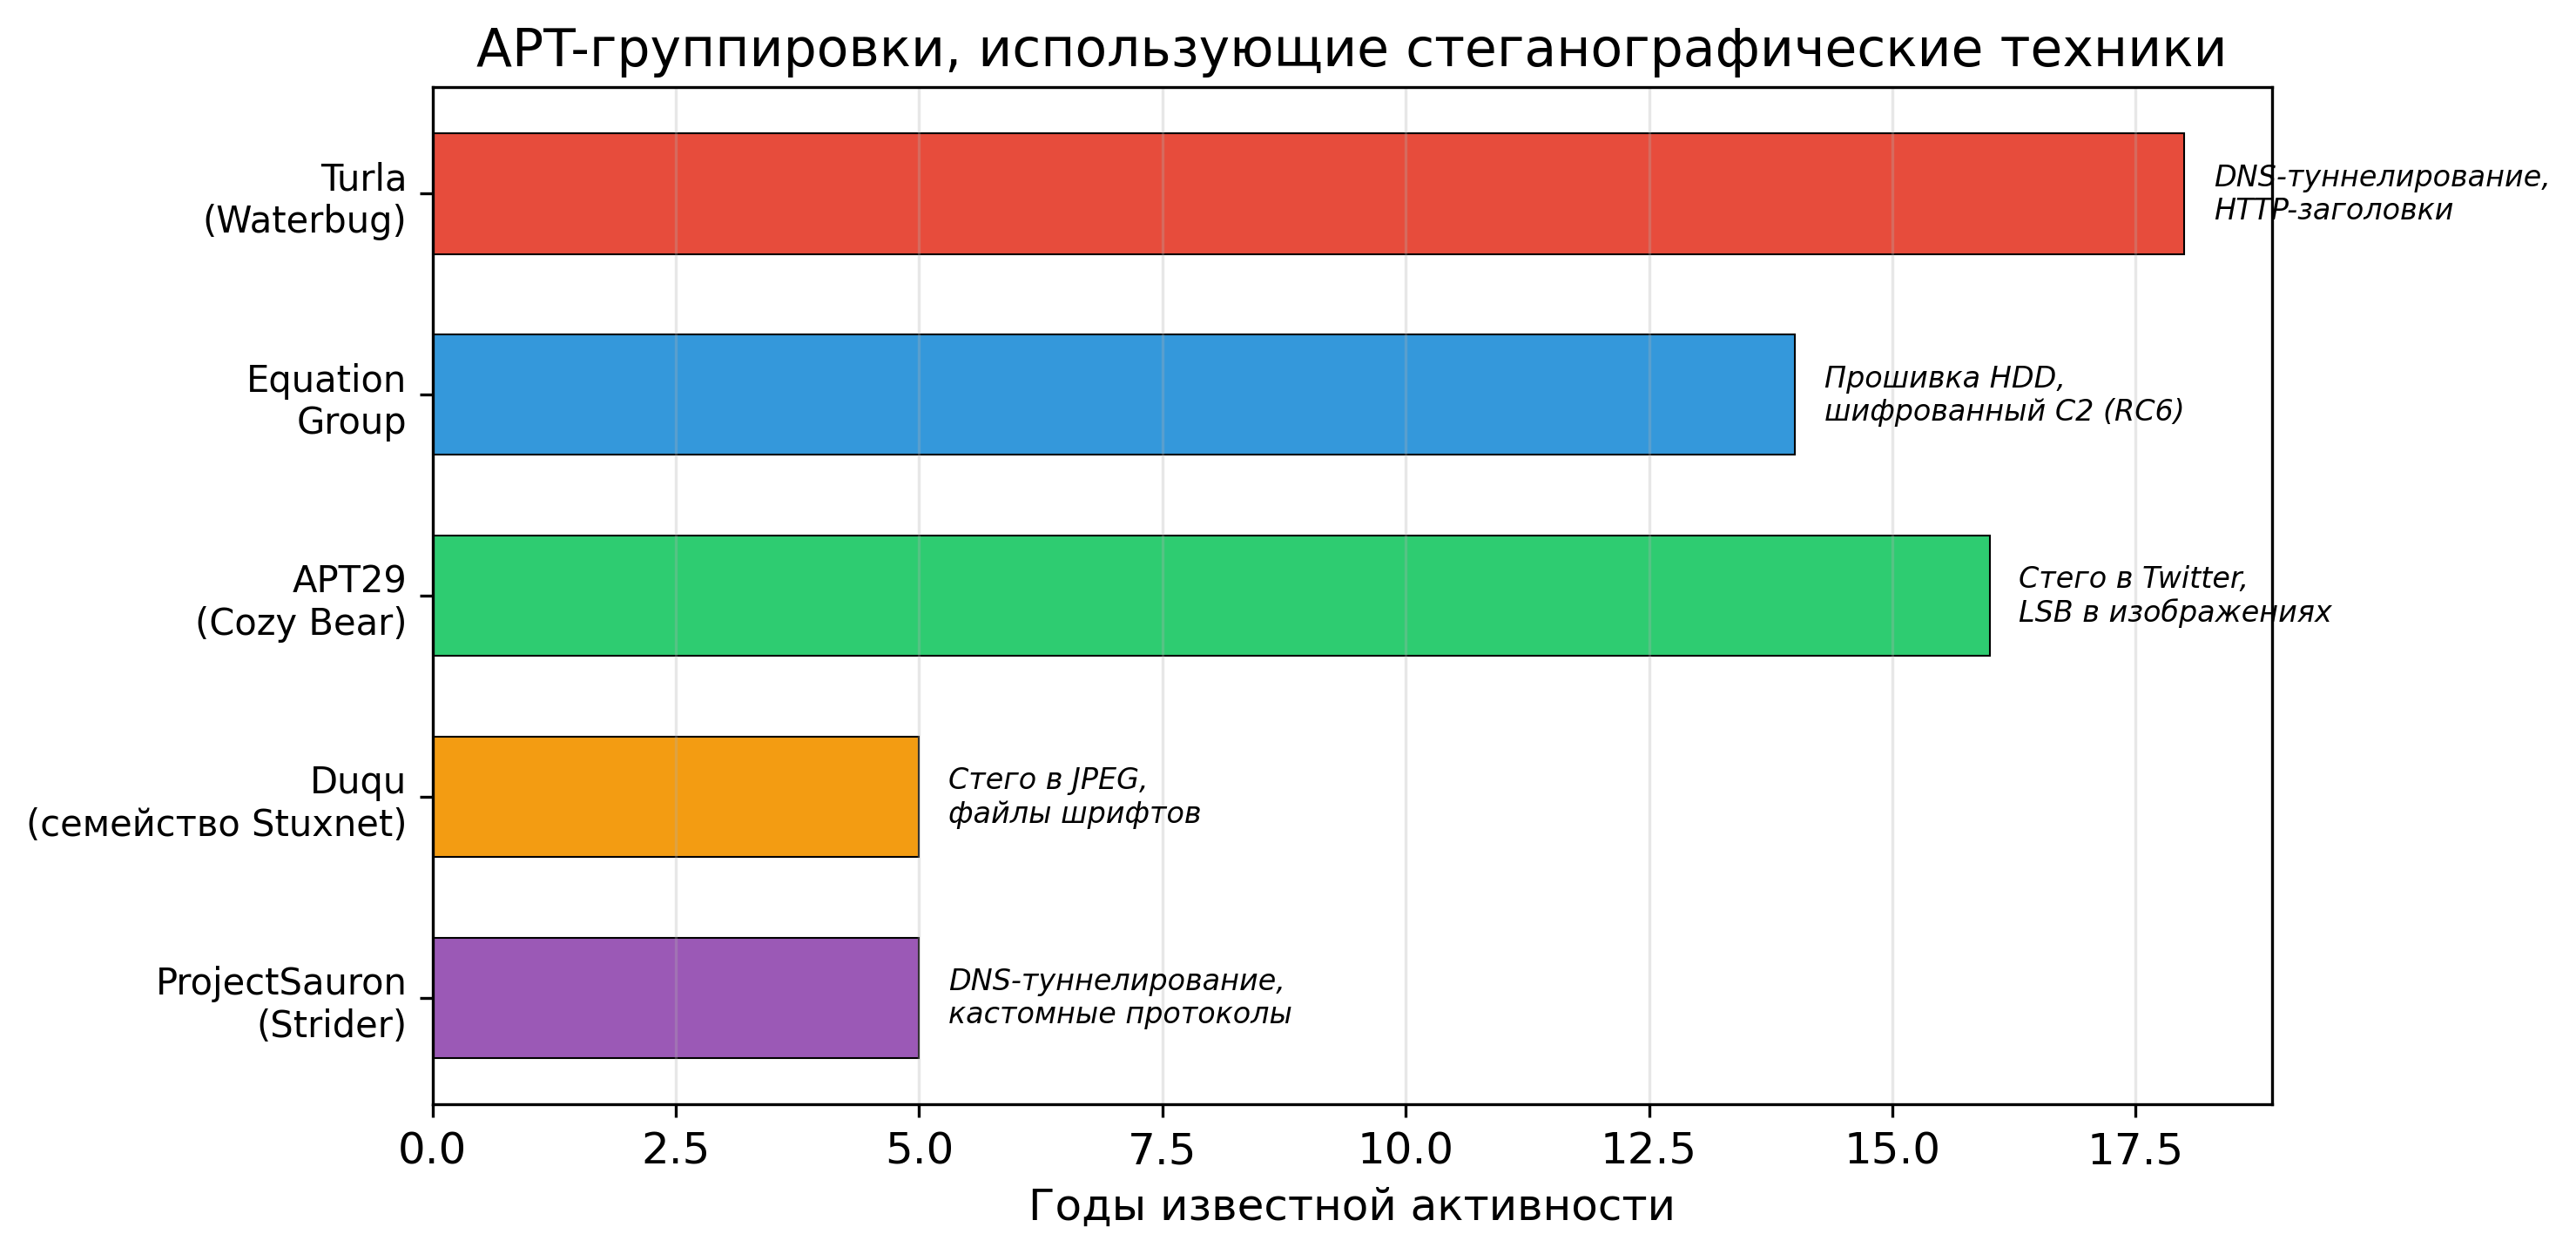
\includegraphics[width=0.9\textwidth]{images/apt_stego.png}
    \caption{APT-группировки, использующие стеганографические техники}
    \label{fig:apt_stego}
\end{figure}

Как видно из диаграммы, некоторые из рассмотренных группировок ведут активную деятельность на протяжении более 15~лет (Turla~--- с 2008~года, Equation Group~--- с 2001~года), что свидетельствует о высокой эффективности стеганографических методов сокрытия и трудности их обнаружения традиционными средствами защиты. Разнообразие применяемых техник~--- от DNS-туннелирования и модификации TCP/IP-заголовков до стеганографии в изображениях~--- указывает на необходимость комплексного подхода к обнаружению, сочетающего статистический анализ, машинное обучение и сигнатурные методы.

Рост популярности стеганографии в сетевых протоколах обусловлен рядом факторов:

\begin{enumerate}[label=\arabic*)]
    \item обход систем глубокого анализа трафика (DPI), основанных на детектировании сигнатур;
    \item способность маскироваться под обычный сетевой трафик, снижая вероятность обнаружения;
    \item отсутствие сквозного шифрования заголовков протоколов TCP/IP, что упрощает манипуляции с ними;
    \item широкий выбор полей и опций, пригодных для стеганографии.
\end{enumerate}

\subsection{Влияние скрытых каналов на безопасность корпоративных сетей}

Скрытые каналы связи (covert channels) были впервые формализованы в работах Lampson (1973)~[17] и разделены на два основных типа: каналы хранения (covert storage channels) и каналы времени (covert timing channels). В контексте сетевых протоколов каналы хранения реализуются через встраивание данных в поля заголовков или полезной нагрузки пакетов, а каналы времени~--- через манипуляцию интервалами передачи пакетов.

Сравнительная характеристика типов скрытых каналов по ключевым параметрам представлена на рисунке~\ref{fig:channel_classification}. Оценка производится по трём критериям: пропускная способность, скрытность и сложность обнаружения.

\begin{figure}[htbp]
    \centering
    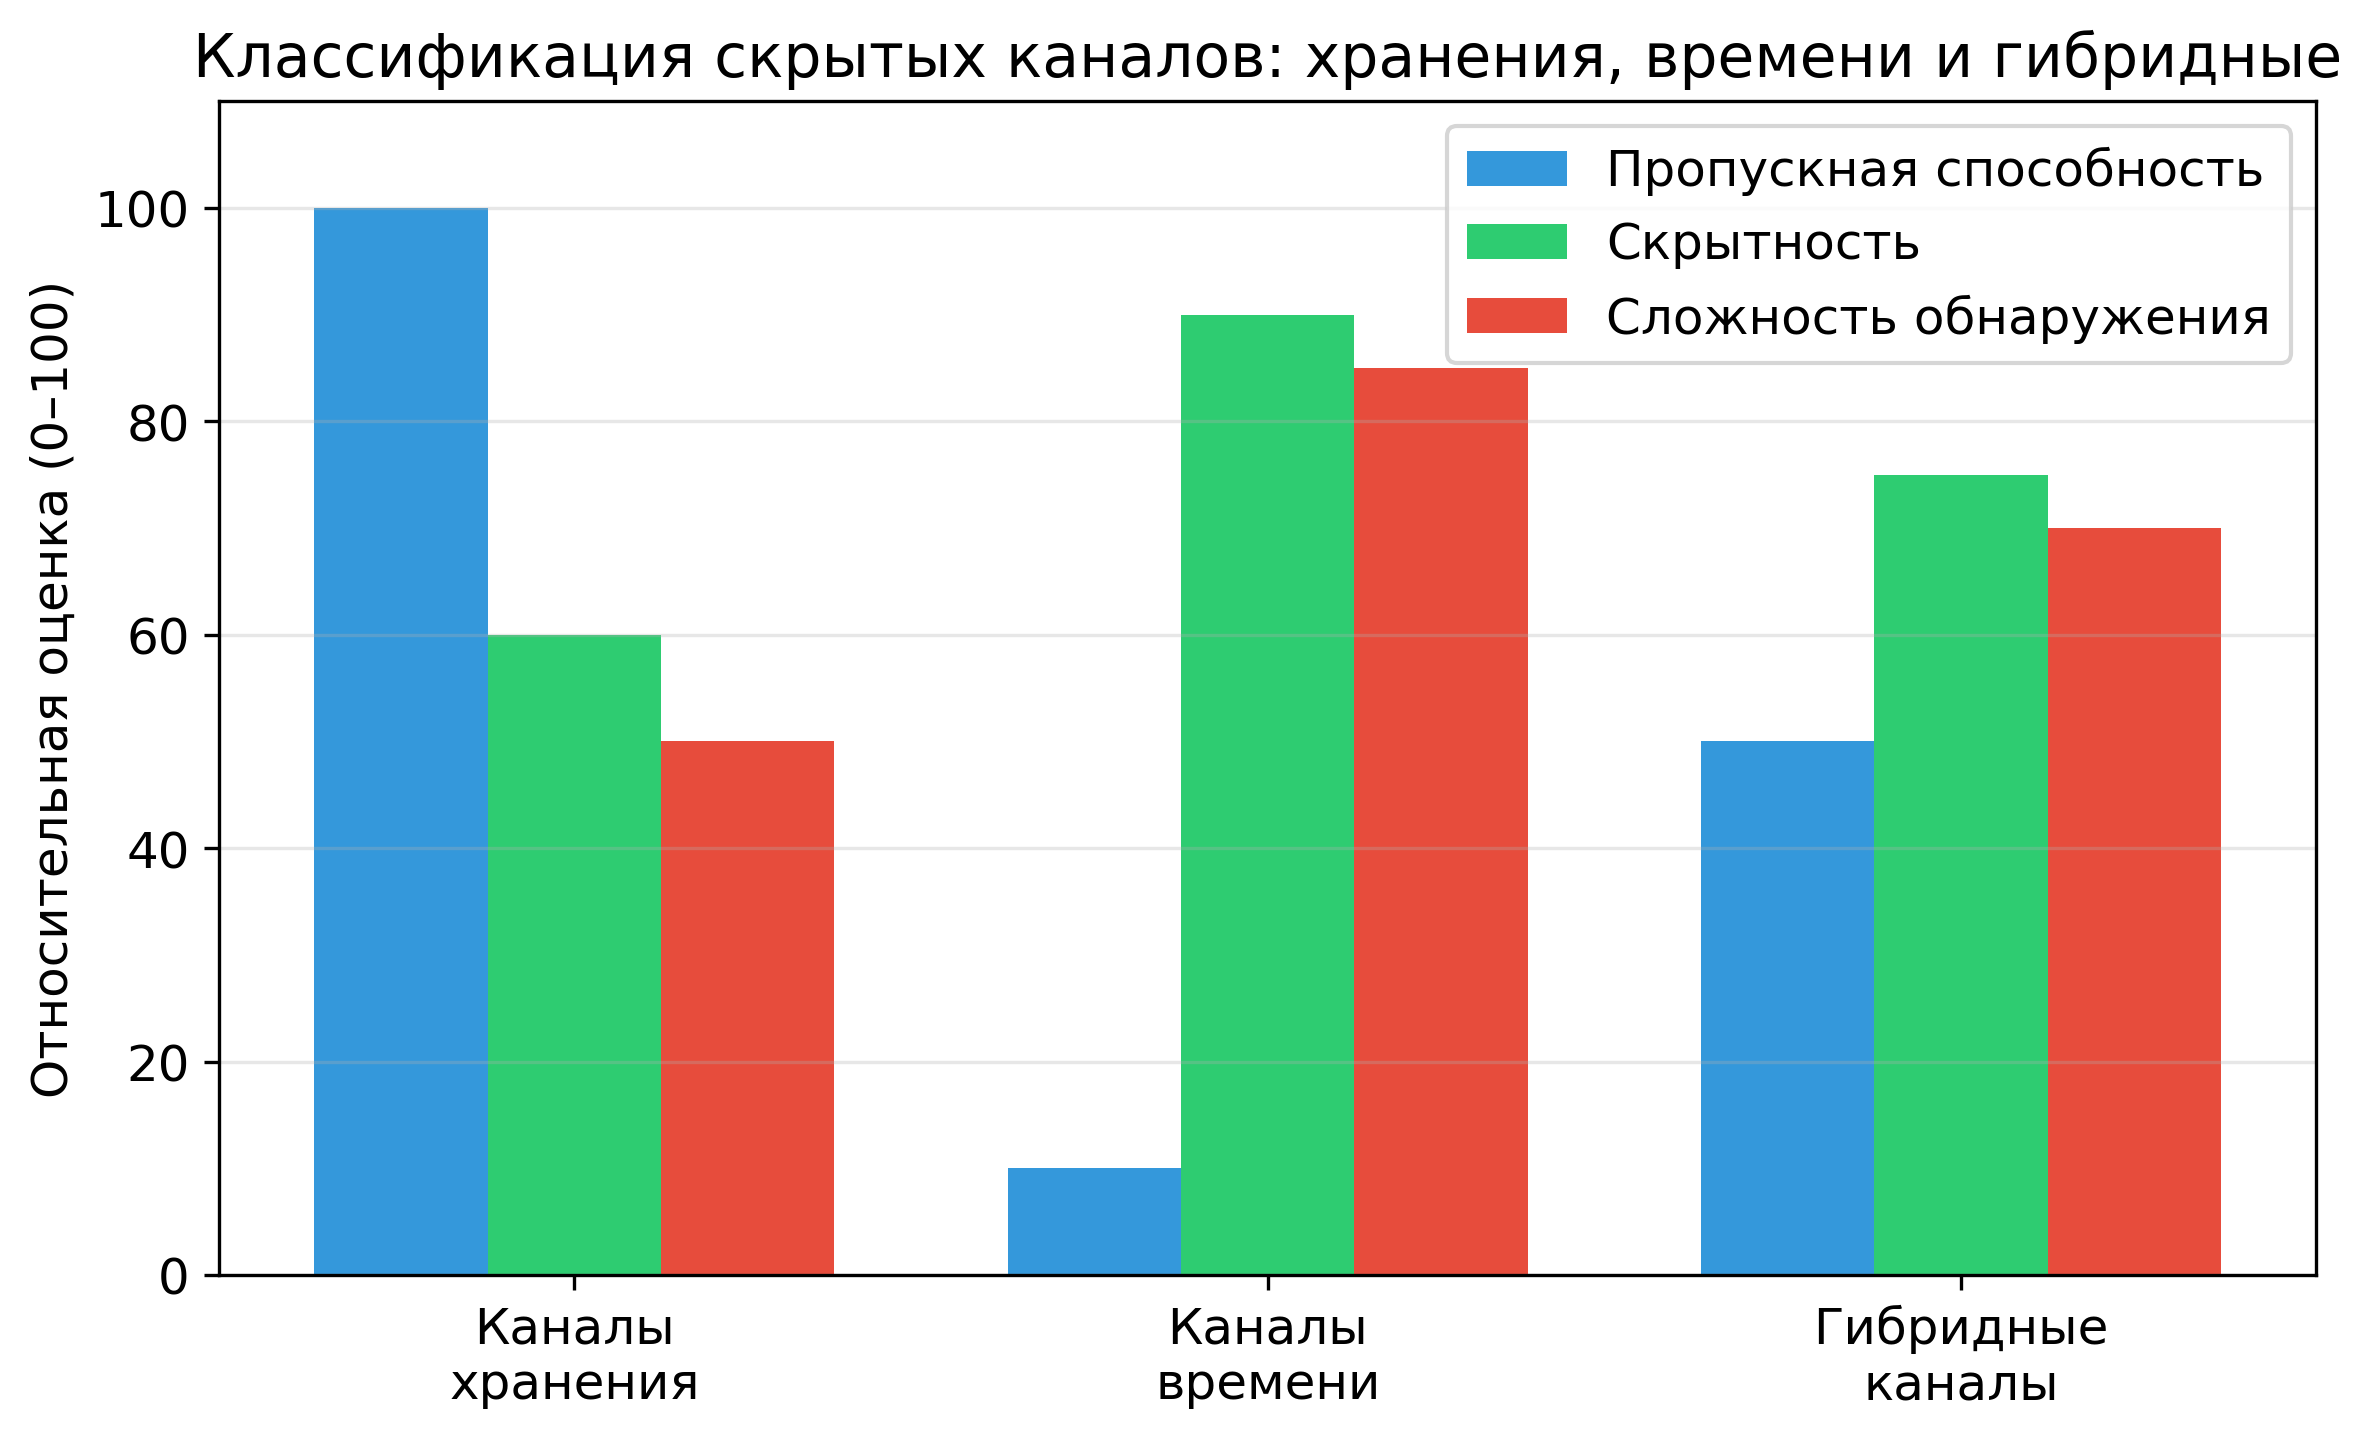
\includegraphics[width=0.8\textwidth]{images/channel_classification.png}
    \caption{Классификация скрытых каналов: хранения, времени и гибридные}
    \label{fig:channel_classification}
\end{figure}

Каналы хранения обладают наибольшей пропускной способностью, поскольку позволяют встраивать данные непосредственно в поля пакетов, однако их скрытность относительно невысока~--- модифицированные поля могут быть выявлены статистическим анализом. Каналы времени, напротив, характеризуются высокой скрытностью и сложностью обнаружения, но их пропускная способность существенно ограничена, так как информация кодируется через межпакетные задержки. Гибридные каналы, комбинирующие оба подхода, представляют компромисс между пропускной способностью и скрытностью, однако их реализация значительно сложнее.

Использование таких скрытых каналов представляет серьёзные риски для безопасности корпоративных сетей, включая:

\begin{enumerate}[label=\arabic*)]
    \item эксфильтрацию конфиденциальных данных в обход систем контроля доступа (NAC) и межсетевых экранов;
    \item реализацию командно-контрольных (C2) каналов для управления вредоносным ПО;
    \item затруднение обнаружения и идентификации атакующих активностей.
\end{enumerate}

Помимо непосредственных технических рисков, скрытые каналы создают значительные проблемы для процессов реагирования на инциденты. При расследовании компрометации организации аналитики, как правило, фокусируются на анализе известных индикаторов компрометации (IoC) --- IP-адресов, доменных имён, хешей файлов. Стеганографические каналы, использующие легитимные протоколы и не создающие новых сетевых соединений, не порождают характерных IoC и могут оставаться незамеченными даже при детальном ретроспективном анализе трафика. Это обстоятельство значительно увеличивает среднее время обнаружения инцидента (Mean Time to Detect, MTTD), которое, по данным отчёта IBM Cost of a Data Breach~[12], составляет 204~дня для атак с использованием продвинутых техник сокрытия.

Кроме того, наличие скрытых каналов в корпоративной сети ставит под сомнение эффективность контрольных мер, основанных на мониторинге сетевого трафика. Системы класса DLP (Data Loss Prevention), контролирующие исходящий трафик на предмет утечки конфиденциальных данных, оказываются неэффективными при стеганографической эксфильтрации, поскольку данные передаются в полях заголовков, не подвергаемых содержательному анализу~[13]. Аналогичным образом, системы SIEM (Security Information and Event Management), агрегирующие журналы событий, не фиксируют манипуляции с полями заголовков на уровне отдельных пакетов.

Таким образом, понимание и обнаружение скрытых каналов является ключевой задачей обеспечения комплексной защиты информационных систем.

\subsection{Нормативно-правовые аспекты обнаружения скрытых каналов}

Проблема обнаружения скрытых каналов в сетевых протоколах имеет не только техническое, но и нормативно-правовое измерение. В Российской Федерации вопросы защиты информации в информационных системах регулируются комплексом нормативных актов и руководящих документов.

Федеральная служба по техническому и экспортному контролю (ФСТЭК России) определяет требования к защите информации в информационных системах различных классов. Приказ ФСТЭК России №~17 от 11~февраля 2013~года <<Об утверждении требований о защите информации, не составляющей государственную тайну, содержащейся в государственных информационных системах>> устанавливает обязательность применения мер по обнаружению вторжений (ОБС) и анализу защищённости (АНЗ) для информационных систем 1-го и 2-го классов защищённости. В контексте данных требований скрытые каналы представляют собой класс угроз, для противодействия которым необходимы специализированные средства анализа.

Приказ ФСТЭК России №~239 от 25~декабря 2017~года <<Об утверждении требований по обеспечению безопасности значимых объектов критической информационной инфраструктуры Российской Федерации>> определяет меры по защите значимых объектов КИИ. Для объектов 1-й категории значимости предусматривается необходимость контроля информационных потоков и обнаружения скрытых каналов утечки информации. Методический документ ФСТЭК <<Меры защиты информации в государственных информационных системах>> конкретизирует данные требования, указывая на необходимость анализа сетевого трафика с целью выявления нехарактерных информационных потоков.

Федеральный закон №~187-ФЗ <<О безопасности критической информационной инфраструктуры Российской Федерации>> от 26~июля 2017~года обязывает субъектов КИИ обеспечивать непрерывность функционирования объектов и информирование ГосСОПКА о компьютерных инцидентах. Использование злоумышленниками стеганографических каналов для управления вредоносным ПО на объектах КИИ создаёт угрозу нарушения их функционирования, что обуславливает необходимость разработки и внедрения средств обнаружения таких каналов.

На международном уровне стандарт ISO/IEC~27001:2022 в рамках контрольных мер приложения~A (A.8.16 <<Monitoring activities>>) предусматривает мониторинг сетевого трафика с целью выявления аномалий, в том числе скрытых каналов. Стандарт NIST~SP~800-53~Rev.~5 включает контрольную меру SC-31 <<Covert Channel Analysis>>, непосредственно адресующую проблему анализа скрытых каналов в информационных системах и рекомендующую проведение систематического анализа системных интерфейсов на предмет наличия скрытых каналов.

Таким образом, разработка инструментов обнаружения стеганографических скрытых каналов в сетевых протоколах является не только научно-исследовательской задачей, но и необходимым условием обеспечения соответствия информационных систем требованиям регуляторов в области информационной безопасности.

\subsection{Роль протоколов TCP/IP как носителей скрытой информации}

Стек протоколов TCP/IP остаётся основным стандартом передачи данных в глобальной сети. Его широкое распространение и отсутствие шифрования некоторых заголовочных полей делают его удобной средой для реализации сетевой стеганографии~[1, 3].

Основными полями и элементами протоколов, подходящими для сокрытия данных, являются:

\begin{enumerate}[label=\arabic*)]
    \item \textbf{IP Identification (IP ID)} --- 16-битное поле в заголовке IPv4 (RFC 791~[3]), предназначенное для идентификации фрагментов пакетов. Использование этого поля позволяет встраивать 2 байта данных на пакет, при этом необходимо учитывать особенности поведения операционной системы, такие как инкрементальное или случайное формирование значения~[3].
    \item \textbf{TCP Initial Sequence Number (ISN)} --- 32-битное поле, устанавливаемое при инициации TCP-соединения (RFC 793~[4]), однако с применением рандомизации (RFC 6528~[18]) для повышения безопасности. Встраивание данных требует аккуратной обработки и обхода защитных механизмов.
    \item \textbf{TCP Timestamp (TSval)} --- 32-битное поле в опции TCP Timestamp (RFC 7323~[7]), используемое для оценки времени прохождения пакетов. Для корректной работы метод должен учитывать политики операционной системы относительно timestamps (например, net.ipv4.tcp\_timestamps = 1).
    \item \textbf{ICMP Echo Request Payload} --- поле данных в ICMP-пакетах (RFC 792~[5]), объёмом до 1472 байт (с учётом MTU Ethernet), предоставляющее значительный объём для скрытия информации, хотя и менее скрытное из-за отсутствия шифрования и возможности анализа размера.
    \item \textbf{DNS QNAME} --- имя доменного запроса в протоколе DNS (RFC 1035~[6]), длина до 255 байт, с возможностью кодирования в base32 и маскировкой под легитимные DNS-запросы.
\end{enumerate}

Существенным фактором, определяющим возможности и ограничения стеганографического использования указанных полей, является различие в поведении операционных систем при формировании значений заголовков пакетов.

В отношении поля IP~ID наблюдаются принципиальные различия между операционными системами. Ядро Linux (начиная с версии 4.1) использует алгоритм генерации IP~ID на основе хеш-функции от адреса назначения, что приводит к формированию отдельной инкрементальной последовательности для каждого уникального адреса. Для пакетов с установленным флагом DF (Don't Fragment) ядро Linux может устанавливать IP~ID в значение~0, что является допустимым согласно RFC~6864~[3]. Операционные системы семейства Windows (начиная с Windows~Vista) используют глобальный инкрементальный счётчик IP~ID, увеличиваемый на единицу для каждого исходящего пакета вне зависимости от адреса назначения. Операционная система FreeBSD реализует случайную генерацию IP~ID с использованием криптографически стойкого генератора. Указанные различия имеют непосредственное значение для стеганографии: замена значения IP~ID на произвольное значение наиболее заметна в среде Windows с её предсказуемой инкрементальной моделью, и наименее заметна в FreeBSD, где значения и без того являются случайными.

В отношении начальных порядковых номеров TCP (ISN) все современные операционные системы реализуют рандомизацию в соответствии с RFC~6528~[18], однако конкретные алгоритмы различаются. Ядро Linux использует функцию SipHash от четвёрки значений (IP-адреса и порты источника и назначения) с добавлением счётчика, инкрементируемого каждые 64~наносекунды. Windows использует аналогичный подход, однако с собственной реализацией хеш-функции и другим интервалом инкрементирования. Для стеганографии в TCP~ISN критическим является тот факт, что полная замена значения ISN нарушает корреляцию между значениями ISN для последовательных соединений к одному серверу, что может быть выявлено при статистическом анализе.

Поведение TCP Timestamp также зависит от операционной системы. В Linux начальное значение TSval формируется на основе значения \texttt{jiffies} --- внутреннего счётчика ядра с частотой, определяемой конфигурацией \texttt{CONFIG\_HZ} (типичные значения~--- 100, 250 или 1000~Гц). Таким образом, TSval инкрементируется с предсказуемой частотой, и любое отклонение от линейного роста может служить индикатором стеганографической модификации. В Windows TCP Timestamp инкрементируется с частотой 100~Гц (шаг 10~мс). Стеганографическая замена TSval на произвольное значение нарушает монотонность последовательности, что является обнаруживаемой аномалией.

Для протокола ICMP различия между ОС проявляются в размере полезной нагрузки по умолчанию: утилита \texttt{ping} в Linux отправляет 56~байт данных (в итоге 64~байта с заголовком ICMP), в Windows~--- 32~байта, а в macOS~--- также 56~байт. Содержимое payload по умолчанию также различается: Linux заполняет его временной меткой и инкрементируемыми байтами, Windows использует повторяющуюся последовательность \texttt{abcdefghijklmnop...}. Стеганографическое использование ICMP payload требует имитации паттерна конкретной ОС для снижения вероятности обнаружения.

Данные поля образуют базу для создания эффективных и скрытных стеганографических каналов в сетевых коммуникациях.

